\chapter{Blend Shape Models}
\label{chap:blendshapemodels}

Facial animation in film is typically done using blend shape models,
as they provide an easy-to-use framework that disallows unnatural facial deformations (unlike e.g.\ freeform deformations),
while also exposing parameters that are intuitively interpretable by animators (unlike e.g.\ generative PCA models).
A blend shape model is a linear, \textbf{semantic parameterization} of a face's range of expressions,
where the individual components (the \textbf{blend shape targets}) are \textquote{core} expressions that are linearly combined to reach a greater range of \textquote{mixed} expressions (the blend shape targets are the \textquote{basis} of the spanned \textquote{expression-space}).
This choice of linear components introduces a semantic interpretability to the model parameters,
as each parameter controls the influence of an intuitive human expression on the resulting model.
The total \textquote{range} of the model depends on the number of used blend shapes,
but in general a blend shape model remains a lossy representation of the human expression-space.

Custom blend shape targets can be chosen depending on the model requirements,
with the \textquote{Facial Action Coding System} (FACS) there also exists a standardized definition of \textquote{components} of facial expressions based on human anatomy.
FACS defines 46 \textquote{action units} that correspond to facial muscle movements (not counting units for general head and eye movement),
which can be realized as delta blend shape targets.

In contrast to skeletal forward and inverse kinematics,
blend shape kinematics does not deal with models made of bone segments and joints,
although the general problem formulations \(x=f(\theta)\) (forward) and \(\theta=f^{-1}(x)\) (inverse) stay the same.

\section{Delta Blend Shape Forward Kinematics}
\label{sec:blendshapeforwardkinematics}

The forward kinematics approach to facial animation using delta blend shape models consists of an animator tuning individual parameters of the model to reach a target expression.
The blend shape model's components are the \textquote{neutral face} \(b_0\) and \(n\) blend shape targets (custom created facial expressions) \(b_1,\dots,b_n\) (\(b_i\) always denotes a regular blend shape target, delta blend shape targets are denoted as \(b_i-b_0\)).
Each \(b_i\) has \(m\) vertices and identical triangulation to allow representation of a target expression as a linear combination of \(b_0,\dots,b_n\).
Every blend shape \(b_i\) \textquote{is a vector of \(m\) stacked vertex positions}:
\[b_i=\begin{pmatrix}
  x_i^{(i)}\\
  \vdots\\
  x_m^{(i)}\\
\end{pmatrix}\in\mathbb{R}^{3m}.\]
Because \(x_i^{(i)}\in\mathbb{R}^3\),
each vertex's three coordinates are contained in \(b_i\) either in packed or interleaved fashion:
\(b_i=(x_1,\dots, x_m, y_1,\dots,y_m, z_1,\dots, z_m)^T\) or \(b_i=(x_1,y_1,z_1,\dots,x_m,y_m,z_m)^T\).
The ordering does not matter, as long as it is identical for every \(b_i\) and the neutral face \(b_0\).

A target expression \(F(w)\) is then generated by setting the \(n\)-dimensional parameter-vector \(w\) for an affine linear combination:
\[F(w)=b_0+\sum\limits_{i=1}^n w_i(b_i-b_0).\]
By combining divergences from the neutral face (\textquote{delta-blend shapes}),
each parameter \(w_i\) can be chosen arbitrarily\footnote{
  Parameters should be chosen from the interval \([0, 1]\).
  For the inverse kinematics problem,
  this range is usually not enforced,
  since the target expression could leave the spanned expression space (for example by opening the mouth too much).
  For slight excesses this shouldn't be a problem,
  but in general the delta blend shape target \(b_i\) is reached fully with weights \(w_j=0\ \forall j\neq i\) and \(w_i=1\),
  so a weight exceeding \(1\) is of undefined quality.
},
while the effective weights \(\alpha_0,\dots,\alpha_n\) for blend shapes \(b_0,\dots,b_n\) still satisfy the affine property \(\sum_{i=0}^n\alpha_i=1\) (which is required,
otherwise the target expression could \textquote{leave} the expression space spanned by the blend shapes,
for example by unwanted scale deformations):
\begin{align*}
  F(w)&=b_0+\sum\limits_{i=1}^{n}w_i(b_i-b_0)\\
  &=b_0+\sum\limits_{i=1}^{n}w_i b_i-\sum\limits_{i=1}^{n}w_i b_0\\
  &=b_0\underbrace{\left(1-\sum\limits_{i=1}^{n}w_i\right)}_{\alpha_0}+\sum\limits_{i=1}^{n}\underbrace{w_i}_{\alpha_i} b_i\\
  \Rightarrow \sum\limits_{i=0}^{n}\alpha_i &= 1-\left(\sum\limits_{i=1}^{n}w_i+\sum\limits_{i=1}^{n}w_i\right)=1
\end{align*}
By combining the delta blend shape vectors \(b_i-b_0\) into a matrix
\[B=[b_1-b_0|\dots|b_n-b_0]\]
with \(B\in\mathbb{R}^{3m\times n}\), the model can be formulated more compactly:
\[F(w)=b_0+Bw.\]

The semantic nature of blend shape models makes animation using this forward approach generally possible for smaller models,
but it becomes inefficient or even impossible for high-quality models with hundreds of parameters\footnote{
  The facial model created for \textquote{Gollum} from \textquote{The Lord of the Rings} uses over \(900\) blend shape targets.~\autocite{computeranimation}
}.

\section{Delta Blend Shape Inverse Kinematics}
\label{sec:blendshapeinversekinematics}

For this reason, animation using the inverse kinematics approach is desirable:
Instead of interacting with individual parameters,
\textquote{markers} or \textquote{manipulators} are placed on the model,
which allow to define the target expression more directly.
Markers positions can be obtained either manually through a user interface which allows direct interaction with the model (like in \autoref{fig:effectorface}) or through facial tracking (see \autoref{chap:performancedrivenfacialanimation}).
The blend shape parameters are then determined to match this target expression as closely as possible.

\begin{figure}[h]
  \centering
  \begin{subfigure}[b]{0.53\textwidth}
	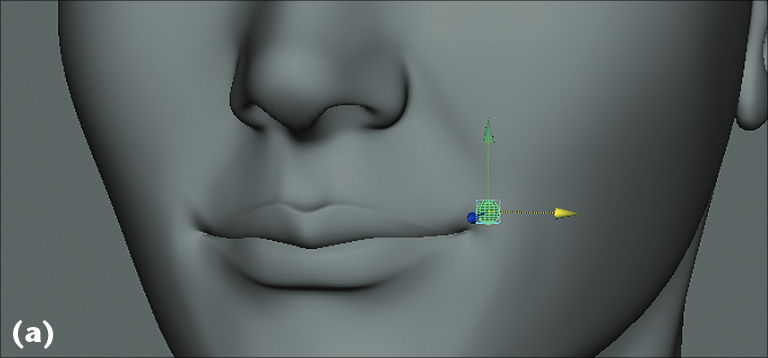
\includegraphics[scale=0.3]{img/effector_face.png}
  \end{subfigure}
  \caption{A marker placed on a facial model.~\autocite{directmanipulationblendshapes}}
  \label{fig:effectorface}
\end{figure}

Placing a marker on the model effectively means choosing a vertex,
whose position should act as a constraint for the face deformation.
Marker \(i\)'s current position is the current vertex position \(x_i\),
which depends on the current model parameters \(w\).
The vertex's target position \(t_i\) can then be defined by moving the marker around.

Determining the model parameters \(w\) to satisfy the marker constraints can be formulated as the following minimization problem:
\[w=\arg\min\limits_w||\overline{B}w-(\overline{t}-\overline{b}_0)||^2=\arg\min\limits_w||\overline{B}w-m||^2,\]
where \(t\) is the vector of all marker's target positions,
\(m\) are the offsets of the target positions from the neutral face (offsets are used because of delta blend shapes) and \(\overline{B}\),
\(\overline{t}\) and \(\overline{b}_0\) correspond to \(B\),
\(t\) and \(b_0\) but only contain the rows belonging to the vertices that are constrained by markers.~\autocite{directmanipulationblendshapes}
This means, \(\overline{B}\) contains \(3\) rows for each placed marker.
Since the direct manipulation allows targeting expressions outside the model's expression space,
an exact solution is generally not possible.
Also, the above minimization problem will be under-constrained in most cases (unless the animator places possibly hundreds of markers),
so additional constraints or regularization terms need to be introduced.

To improve temporal continuity of the animation, weight differences between updates can be minimized by introducing \(\alpha||w-w_0||^2\) to the problem,
where \(w_0\) are the previous weights:~\autocite{directmanipulationblendshapes}
\[w=\arg\min\limits_w||\overline{B}w-m||^2+\alpha||w-w_0||^2,\]
Lewis and Anjyo add \(\mu||w||^2\) as another regularization term,
with the intention to oppose \textquote{extreme} solutions,
for example caused by weight growth due to numerical errors in \textquote{oscillating} animations:~\autocite{directmanipulationblendshapes}
\[w=\arg\min\limits_w||\overline{B}w-m||^2+\alpha||w-w_0||^2+\mu||w||^2.\]
This term is also important since the weights \(w\) are not constrained to \([0, 1]\) for the inverse problem (at least not in this solution).

The parameters \(\alpha\) and \(\mu\) are set to small values to not significantly alter the main objective,
Lewis and Anjyo use \(\alpha=0.1\) and \(\mu=0.001\).~\autocite{directmanipulationblendshapes}

\section{Solving the Inverse Kinematics Minimization Problem}
\label{sec:solvingblendshapeinversekinematics}

The goal is the minimization of
\[||\overline{B}w-m||^2+\alpha||w-w_0||^2+\mu||w||^2,\]
which is quadratic in \(w\).
Since we are using the euclidian norm,
it follows that
\[||x||^2=\sqrt{x_1^2+\dots+x_n^2}^2=x_1^2+\dots+x_n^2=x^T x\]
for \(x\in\mathbb{R}^n\), which allows us to rewrite the term as
\begin{align*}
  &(\overline{B}w-m)^T(\overline{B}w-m)+\alpha(w-w_0)^T(w-w_0)+\mu w^T w\\
  =\ &(w^T \overline{B}\,^T \overline{B}w-2w^T \overline{B}\,^T m+m^T m)\\
  &+\alpha(w^T w-2w^T w_0+w_0^T w_0)\\
  &+\mu(w^T w).
\end{align*}
Deriving this (using some slightly sketchy matrix differential notation\footnote{
  Sketchy example:\\
  \(d\phi(w)=d(w^T\overline{B}\,^T\overline{B}w)=(dw)^T\overline{B}\,^T\overline{B}w+w^T\overline{B}\,^T\overline{B}(dw)=2w^T\overline{B}\,^T\overline{B}(dw)\Leftrightarrow\frac{d\phi}{dw}=2\overline{B}\,^T\overline{B}w\)
}) leads to the following derivative:
\[2\overline{B}\,^T\overline{B}w-2\overline{B}\,^T m+2\alpha w-2\alpha w_0+2\mu w.\]
Solving for \(0\) to find the local extremum leads to
\begin{align*}
  2\overline{B}\,^T\overline{B}w+2\alpha w+2\mu w&=2\overline{B}\,^T m+2\alpha w_0\\
  \Leftrightarrow\left(\overline{B}\,^T\overline{B}+(\alpha+\mu)I\right)w&=\overline{B}\,^T m+\alpha w_0,
\end{align*}
which is a \(n\times n\) linear system (\(n\) is the number of blend shapes/model parameters),
where \(I\in\mathbb{R}^{n\times n}\) is the identity matrix.
The above condition is sufficient, since the problem is convex.

Because \(\overline{B}\,^T\overline{B}\) and \((\alpha+\mu)I\) are both (usually) positive definite\footnote{
  For a matrix \(A\), \(A^T A\) is positive definite if \(Ax\neq 0\) for any non-zero vector \(x\),
  since \(x^T A^T Ax=(Ax)^T(Ax)=||Ax||^2\).
  This is probably true for \(\overline{B}\),
  since \(\overline{B}\)'s columns (the partial delta blend shape targets) should be linearly independent.
}\ \footnote{
  The identity matrix and its scalar multiples are positive definite.
} and equal to their (conjugate\footnote{
  We only deal with real numbers (coordinates from \(\mathbb{R}^3\)).
}) transposes\footnote{
  \((A^T A)^T=A^T(A^T)^T=A^T A\).
}, an efficient Cholesky solver can be applied to obtain \(w\).~\autocite{computeranimation}

\subsection{Inverse Kinematics Instability}
\label{subsec:pseudoinverseinstability}

Disregarding implementation-specific numerical instabilities and assuming that \(\overline{B}\) is invertible because all delta blend shape targets are linearly independent\footnote{
  If \(\exists\ i, w: b_i = \sum\limits_{j\neq i} w_j b_j\), \(b_i\) can be removed, as it does not add information to the model.
} (so \(\overline{B}\) has full rank),
we have the following equivalence:

\[
  \left(\overline{B}\,^T\overline{B}+(\alpha+\mu)I\right)w=\overline{B}\,^T m+\alpha w_0
  \Leftrightarrow w=\left(\overline{B}\,^T\overline{B}+(\alpha+\mu)I\right)^{-1}\left(\overline{B}\,^T m+\alpha w_0\right)
\]

This is a (regularized) Moore-Penrose pseudo-inverse\footnote{
  This is only true if \(\overline{B}\)'s columns are linearly independent, which I will assume from now on.
  Under these circumstances, it follows for a full-rank matrix \(A\):
  \begin{align*}
    A&=U\Sigma V^T=U\left((\Sigma^+)^T\Sigma\right)\Sigma V^T=U(\Sigma^+)^T (V^T V)\Sigma (U^T U)\Sigma V^T\\
    &=(V\Sigma^+ U^T)^T(U\Sigma V^T)^T(U\Sigma V^T)=\left((U\Sigma V^T)^+\right)^T(U\Sigma V^T)^T(U\Sigma V^T)\\
    &=(A^+)^T A^T A\Leftrightarrow A^T=(A^T A) A^+\Leftrightarrow A^+=(A^T A)^{-1}A^T.
  \end{align*}
  Full rank is required for the property \((\Sigma^+)^T\Sigma=I\).
} or \textquote{damped-least-squares} method:
If we set \(\alpha=0\) and \(\mu=0\) we obtain

\[w=\left(\overline{B}\,^T\overline{B}\right)^{-1}\overline{B}\,^T m=\overline{B}\,^+ m.\]

This can lead to instabilities when \textquote{dragging} or animating a placed marker/constraint:~\autocite{transpositiondirectmanipulationblendshapes}
If we expand our forward kinematics problem \(F(w)=b_0+Bw\) using a singular value decomposition, we end up with

\[F(w)=b_0+U\Sigma V^T w,\]

where the largest singular values in \(\Sigma\) will have the most influence on the generated facial expression.
These are the values that should mainly be used to solve the inverse kinematics problem.

Now, looking at the singular value decomposition of the unregularized inverse kinematics problem \(w=\overline{B}\,^+ m\), we obtain

\[w=(U\Sigma V^T)^+ m=(V^T)^+\Sigma^+U^+ m=V\Sigma^+U^T m,\]

because \(V\) and \(U\) are orthogonal matrices\footnote{
  \(U^+=U^{-1}=U^T\).
}.

Since we take the pseudo-inverse \(\Sigma^+\),
the non-zero diagonal entries of \(\Sigma\) are inverted,
which means this inverse kinematics solution is influenced strongly by the smaller singular values from the forward kinematics problem.
In consequence, the facial deformations produced to satisfy a marker constraint might also occur outside this marker's local environment\footnote{
  In some cases this might be even desirable,
  for example when a smile produces deformations in the eye-region,
  but this makes the model slightly unpredictable.
}, which could lead to inconsistencies during animation.

A possible solution is given by the transposition-based solution of the inverse kinematics problem.~\autocite{transpositiondirectmanipulationblendshapes}~\autocite{jacobiantranspose}

\section{Corrective and Intermediate Blend Shapes}
\label{sec:correctiveblendshapes}

Although the \textquote{basis vectors} of the spanned expression space (the blend shape targets) are valid facial expressions,
arbitrary linear combinations can still produce unnatural anomalies.

\begin{figure}[h]
  \centering
  \begin{subfigure}[b]{0.25\textwidth}
	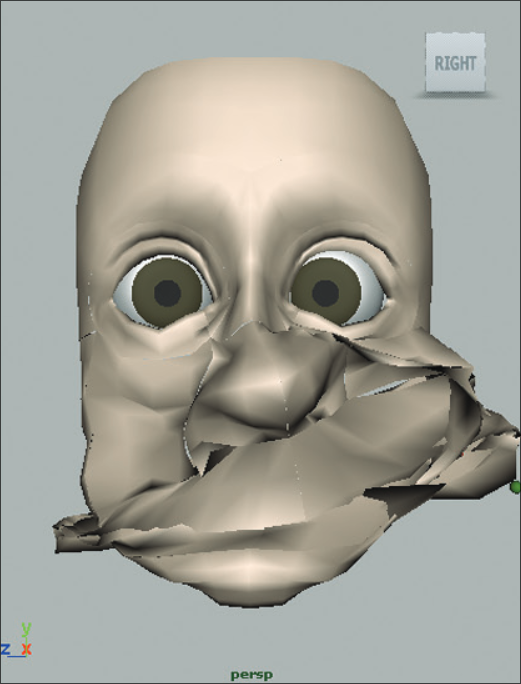
\includegraphics[scale=0.2]{img/unconstrained_weights.png}
  \end{subfigure}
  \caption{Consequences of unconstrained blend shape weights.~\autocite{directmanipulationblendshapes}}
  \label{fig:unconstrainedweights}
\end{figure}

For this reason, \textquote{corrective} blend shapes are used:
By adding blend shape targets with additional weights (not part of the manual model parameters) that depend on other weights,
anomalies caused by special weight combinations can be fixed.

For example, if an anomaly occurs when activating weights \(w_j\) and \(w_k\) for blend shape targets \(b_j\) and \(b_k\),
a corrective blend shape \(b_{(j,k)}\) (\textit{not} in delta blend shape form!) can be modeled for the expression produced by the weights \(w_j=w_k=1\) and \(w_i=0\ \forall i\notin\{j, k\}\).
By setting the weight to \(w_{(j,k)}=w_j\cdot w_k\), the blend shape automatically activates when both \(b_j\) and \(b_k\) become active.

The resulting blend shape model is quadratic with respect to its parameters \(w\):
\begin{align*}
  F_C(w)&=F(w)+\sum\limits_{(i,j)\in C}w_{(i,j)} b_{(i,j)}\\
      &=b_0+\sum\limits_{i=1}^{n}w_i(b_i-b_0)+\sum\limits_{(i,j)\in C}w_i w_j b_{(i,j)},
\end{align*}
where \(C=\{1,\dots,n\}\times\{1,\dots,n\}\) and \(b_{(i,j)}\) denotes the corrective blend shape for blend shape targets \(b_i\) and \(b_j\).
Because of the quadratic nature of this model,
the inverse kinematics problem can no longer be solved by a simple convex optimization.
A possible solution for the quadratic case is given in~\autocite{nonconvexblendshapes},
although corrective blend shapes could also be applied in a third-order fashion or higher (correcting anomalies caused by three or more overlapping blend shape targets).

Another problem arises from the linear nature of the blend shape model:
Certain rotational movements like closing eyelids or eye rotations can only be represented in a linear fashion.
When animating an eyeball movement (like a gaze from center to right),
the eyeball will loose a part of its volume in the first half of the animation and regain it in the second half,
since each individual vertex can only move in a straight line.
To solve this problem, \textquote{intermediate} blend shapes are used:
An additional blend shape target is modeled for a single (or multiple) intermediate animation state(s),
leading to a piecewise linear interpolation/approximation (see \autoref{fig:combinationvsintermediate}).

\begin{figure}[h]
  \centering
  \begin{subfigure}[b]{0.45\textwidth}
	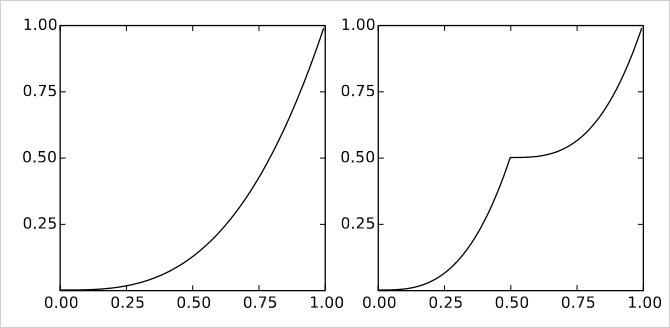
\includegraphics[scale=0.3]{img/combination_vs_intermediate.png}
  \end{subfigure}
  \caption{Corrective blend shapes lead to smooth interpolation that becomes significant if all weights approach \(1\) (left),
    intermediate blend shapes lead to non-smooth interpolation (right).~\autocite{practicetheoryblendshapes}
  }
  \label{fig:combinationvsintermediate}
\end{figure}

This approach can be handled by the in \autoref{sec:blendshapeinversekinematics} described inverse kinematics solution,
as intermediate blend shapes are just appended to the existing linear model.

\section{Combining Skeletal and Blend Shape Animation}
\label{sec:combiningskeletalandblendshapes}

Instead of using intermediate blend shapes to better approximate rotational deformations,
certain facial movements like eye-, eyelid- or jaw rotations can be modeled using skeletal animation and skinning\footnote{
  \textquote{Skinning} is the translation of abstract bone movements into actual skin/vertex movements.
}.
This does not require modeling all facial animation using bones,
as blend shape animation and skeletal animation can be combined.

To achieve this, the blend shape inverse kinematics problem is solved first,
as the deformations caused by skinning do not match the blend shape targets.
The skeletal inverse kinematics problem can be solved later,
because vertex deformations caused by the blend shape model do not modify bone positions.

Although this approach might achieve better performance with rotational movement,
the resulting expressions loose some control,
as the interactions between blend shape and skinning deformations are unclear\footnote{
  It is unclear to me if this model is viable.
}.

A different combinational model is possible by applying corrective blend shapes to a primarily skeleton-based model:
In cases where memory availability is low,
skeletal models may be preferred over blend shape models\footnote{
  Skeletal models are more taxing on CPU/GPU computations,
  since skinning is more computationally expensive than linear interpolation.
  Blend shape models are more taxing on CPU/GPU memory (especially for detailed models with many blend shapes or situtations with many different characters with their own blend shapes),
  since the face is stored many times with different deformations (although data blend shapes help here, as the localized deformations lead to sparse delta blend shape targets).
}.
To still achieve realistic skin movement (which might be hard only through skinning),
corrective blend shapes can be applied after the skinning,
with weights depending on certain joint angles.
In that case, only skeletal inverse kinematics is involved.
